\section{Introduction}
\label{sec:intro}
We introduce a new primitive, that of public-key, IV-based authenticated-encryption with associated data. The genesis of this primitive came from considering the construction of a public-key encryption scheme via the KEM-DEM paradigm, using an off-the-shelf symmetric-key, IV-based AEAD scheme for the DEM.  The latter turns a plaintext message~$M$ into a ciphertext~$C$ under control of a key~$K$, associated data~$\header$ and initial value (IV)~$\pubiv$, written $C \gets \enc_{K}^{\header,\pubiv}(M)$.  In a KEM-DEM construction, the key~$K$ is produced by a (randomized) key-encapsulation algorithm~$(K,X)\getsr\encap_\pk$, where the encapsulation~$X$ is used by the receiver to recover~$K$.  

The associated data input (AD) of the underlying AEAD scheme can be surfaced as an input to the KEM-DEM construction, resulting in a PKE scheme with ``labels'', the name given in previous works to AD in the public-key setting. \tsnote{Kenny thinks there may be some useful distinctions between labels as used in PKE literature, and AD as used the symmetric encryption literature.}  The IV input can be fixed to any particular value, because the key~$K$ that is produced by the encapsulation scheme is fresh each time the KEM-DEM construction is called.  For sake of argument, however let's say that we want a proper IV for the AEAD scheme.  \tsnote{Maybe you don't trust encapsulation to produce full-entropy keys?  Intuitively, it is better to have a mediocre key and a mediocre IV than a mediocre key and a fixed IV.}  Then there are a few options for its origin.

\begin{figure}[h]
\begin{center}
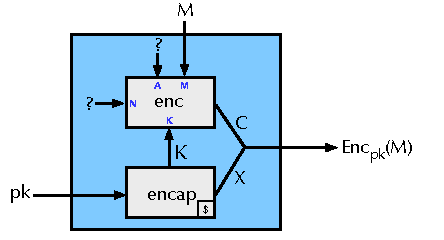
\includegraphics[scale=1.2]{kem-dem.pdf}
\caption{The motivating question: how to build (labeled) public-key encryption, via KEM-DEM, over an IV-based AEAD scheme and a conventional KEM scheme.}
\label{fig:kem-example}
\end{center}
\end{figure}

The first is to demand that the KEM-scheme produces an appropriate IV.  One way to handle this is to define a new type of KEM primitive that includes an algorithm for creating IVs, along with the usual encapsulation and decapsulation algorithms.  Alternatively, we could define a new kind of encapulation algorithm that returns a triple $(K,X,\pubiv)$.  In this case, the algorithm~$\encap$ may need to be both randomized (for generation of~$K$) \emph{and} stateful, if~$\pubiv$ must be a nonce.  (If the underlying AEAD scheme remains secure when~$\pubiv$ is a nonce only with high probability, then $\encap$ need not be stateful.)  Either way, the public-key encryption scheme that results from the KEM-DEM construction remains randomized.  See the left panel of Figure~\ref{fig:kem-dem options} for a psuedocode description of this construction.  Note that we must send~$\pubiv$ as part of the ciphertext (in order to make decrpytion possible), and we choose not to require that~$\pubiv$ be recoverable from~$X$, in order to cleanly separate the encapsulated secret key~$K$ from the public IV.

Although some syntactic changes are required to the standard KEM formalism, it seems unlikely that this option will provide any surprises.  As long as the encapsulation scheme generates~$\pubiv$ in a way that is appropriate for the underlying symmetric AEAD scheme, security statements for the KEM-DEM construction should be straightforward.

\begin{figure}
\begin{center}
\hfpagesss{.25}{.25}{.25}
{
\underline{$\Encprim{\pk}{}{\header, M}$}:\\[2pt]
$(K,X,\pubiv) \getsr \encap_\pk()$\\
$C \gets \encprim{K}{}{\header,\pubiv,M}$\\
Return $(X,N,C)$

\medskip
\underline{$\Decprim{\sk}{}{\header,X,N,C}$}:\\[2pt]
$K \gets \decap_\sk(X)$\\
$M \gets \decprim{K}{}{\header,\pubiv,C}$\\
Return $M$
}
{
\underline{$\Encprim{\pk}{}{\header,\pubiv,M}$}:\\[2pt]
$(K,X) \getsr \encap_\pk()$\\
$C \gets \encprim{K}{}{\header,\pubiv,M}$\\
Return $(X,C)$

\medskip
\underline{$\Decprim{\sk}{}{\header,\pubiv,X,C}$}:\\[2pt]
$K \gets \decap_\sk(X)$\\
$M \gets \decprim{K}{}{\header,\pubiv,C}$\\
Return $M$

}
{
\underline{$\Encprim{\pk}{}{\header,\pubiv,\seciv,M}$}:\\[2pt]
$(K,X) \gets \encap_{\pk}(\header,\pubiv,\seciv)$\\
$C \gets \encprim{K}{}{\header,\pubiv,M \concat \seciv}$\\
Return $(X,C)$

\medskip
\underline{$\Decprim{\sk}{}{\header,\pubiv,X,C}$}:\\[2pt]
$K \gets \decap_\sk(X)$\\
$M \concat \seciv \gets \decprim{K}{}{\header,\pubiv,C}$\\
Return $(\seciv,M)$
}
\caption{Potential KEM-DEM constructions of PKE using an symmetric-key IV-based AEAD scheme $(\enc,\dec)$. \textbf{Left:} Randomized or stateful scheme, in which the encapsulation algorithm generates the IV.  \textbf{Center:} Randomized scheme, in which the IV is surfaced.  \textbf{Right:} Deterministic scheme, in which the externally provided IV is separated into public and private components. The leftmost and rightmost schemes require new syntax for the encapsulation (and decapsulation) algorithms.}
%\tsnote{An actual construction that does a bit more appears in Section~\ref{sec:constructions}}
\label{fig:kem-dem options}
\end{center}
\end{figure}


\paragraph{IV-based PKE(AD). }
A second option is to follow the what has been done in the symmetric setting, and surface the IV (and the associated data) as inputs to encryption; see the center panel of Figure~\ref{fig:kem-dem options}.  
This shifts the requirements for IV generation to the calling environment and, in the KEM-DEM construction under consideration, allows the encapsulation algorithm~$\encap$ to attend to its traditional goals.  %We call any scheme that explicitly takes an IV as input \emph{IV-based}.  

The resulting \emph{IV-based} public-key encryption scheme is still randomized, because $\encap$ is.  In some settings this may be appropriate.  For example, when the calling environment is not trusted to generate (and keep private) randomness to be used by encapsulation, but can provide a reliable counter for the AEAD scheme.  \tsnote{What's a solid example of this?  HSMs accessed by many parties via a fixed API?  Cloud servers that don't know the clients and use TCP sequence number as counter}  In general, however, it seems cumbersome to have IV-based encryption that is also internally randomized.  
%And in applications in which the calling environment \emph{can} be trusted to generate a random IV for the underlying symmetric-key AEAD scheme, then it can provide randomness for other needs, too.
Thus, we consider a third option, that of building a \emph{deterministic} public-key encryption scheme via a KEM-DEM construction over a \emph{deterministic} KEM and an IV-based symmetric-key AEAD scheme.  See the right panel of Figure~\ref{fig:kem-dem options} for details.  


When the scheme is made deterministic, no reasonable security seems achievable when the all inputs are known by the adversary.  So for our fully deterministic construction, we separate the IV into public and secret components $(\pubiv,\seciv)$.   
Note that we do not necessarilly demand that~$S$ be uniformly random.  However, we will require that $(N,S)$ be non-repeating and have a reasonable amount of min-entropy, and that~$S$ be treated as private data. \tsnote{Should~$\seciv$ be recoverable?}  For example, $N$~might be a counter, and~$S$ some function of a password.  We will see simple constructions in the random-oracle model in which this will suffice. As expected, the security of the construction will depend on the min-entropy in $(N,S)$. \tsnote{Standard-model instantiations, in which encapsulation uses a randomness extractor? I think you can publish the extractor key with the public key.}


\paragraph{Syntactic and security requirements on encapsulation. }  The first and last options require obvious syntatic changes to KEM-scheme syntax, as shown in Figure~\ref{fig:kem-dem options}. The deterministic option will also require new security notions for KEM schemes; in particular, a kind of nonce-based KEM security will be needed.  Informally, we will require that the output $(K,X)\gets\encap_{\pk}(A,N,S)$ be indistinguishable from $(R,X)$ where~$R$ is a uniform key for the underlying symmetric AEAD scheme.  This will be required only for adversaries that respect some min-entropy bound on the distribution of $(N,S)$. \tsnote{Not sure how the single-query vs.\ multiple-query issue plays out here.  Seems like you should be able to to have~$S$ be a single password that is used with multiple nonces~$N$ during a session.}

\paragraph{Prior work on PKE with associated data. } \tsnote{Definitely some work to consider.  Start with Shoup's paper: \texttt{http://www.shoup.net/papers/kdm-cca2.pdf}.  What problems has labeled PKE been used to solve?}

\paragraph{Prior work on deterministic PKE. } \tsnote{Which prior deterministic PKE schemes can be seen as examples or special cases of this new primitive? Lots of work in this area over the past 5-7 years. Security notions will likely be different, as we can allow the adversary to have the public key throughout the experiment, and there are nonces.  Should check into hedged encryption, too.}

\paragraph{Prior work on IV-based/deterministic KEM schemes. } \tsnote{I don't know if anyone has considered deterministic KEMs, but I'm guessing that this is a new primitive, too.  KEMs with associated data (``labels'') have been considered.  See H.\ Krawczyk, K.\ G.\ Paterson, and H.\ Wee, ``On the security of the TLS protocol: A systematic analysis'' and J.\ Jonsson and B.\ S.\ Kaliski. ``On the security of RSA encryption in TLS''}

\paragraph{Prior work on password-based encryption. } \tsnote{I don't know the password-based encryption literature very well.  Start with Bellare, Ristenpart, Tessaro and work backwards.}

\paragraph{Applications. } \tsnote{This is a big question! Nonce could be used by server to prevent replay attacks, and password provides a way to do client authentication(?)}
